
\section{Results}

\begin{figure}
\centering
\begin{tabular}{cc}
\subfloat {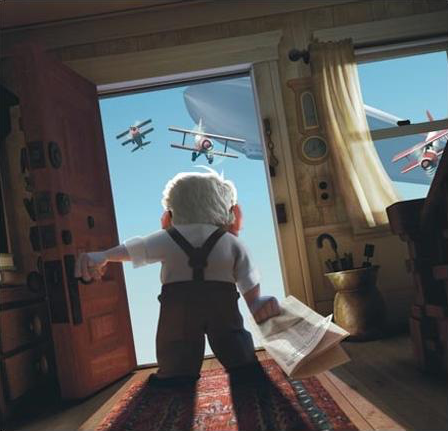
\includegraphics[width=4cm]{images/original_2}} & 
\subfloat {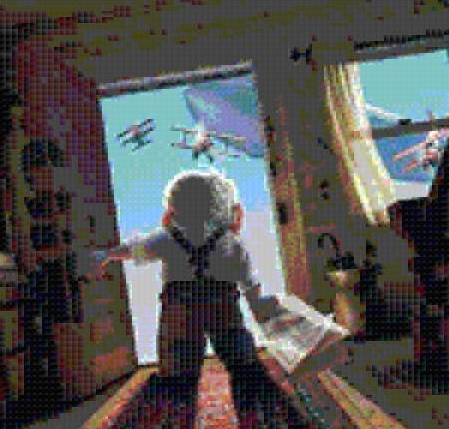
\includegraphics[width=4cm]{images/reconstructed_2}} & 
\end{tabular}
\caption{Visual comparison of original and reconstructed image.}
\label{fig:compare_images}
\end{figure}


We tested the compression algorithm with 100 jpeg-images which were not in the training set and get a mean error of 0.0086 and a compression rate of 0.0094. 
We also tested with 100 images which were all in the training set and the mean error was 0.0082 and the compression rate 0.0092. 
%Time for everything: 907.7797 \newline
%Average quadratic error: 0.0086154 \newline
%Average compression rate: 0.0094089 \newline
%Average inverse for sum compression/error 55.4806 \newline


\newline
%and with 100 images which are all in the training set:\newline
%Time for everything: 873.8136 \newline
%Average quadratic error: 0.008281 \newline
%Average compression rate: 0.0092095 \newline
%Average inverse for sum compression/error 57.174
%\newline
Figure~\ref{fig:compare_images} shows an example image before any compression on the left and the reconstructed image after compression on the right. 
\newline
We also tried to do the training directly on the actual image only. The results were worse than the pre-training. The compression rate was the same, but the mean error was 0.173. This is almost 2 orders of magnitude more than with pre-training.
%Time for everything: 44.1702
%Average quadratic error: 0.17375
%Average compression rate: 0.0086164
%Average inverse for sum compression/error 5.4836

\begin{figure}[tbp]
  \centering
  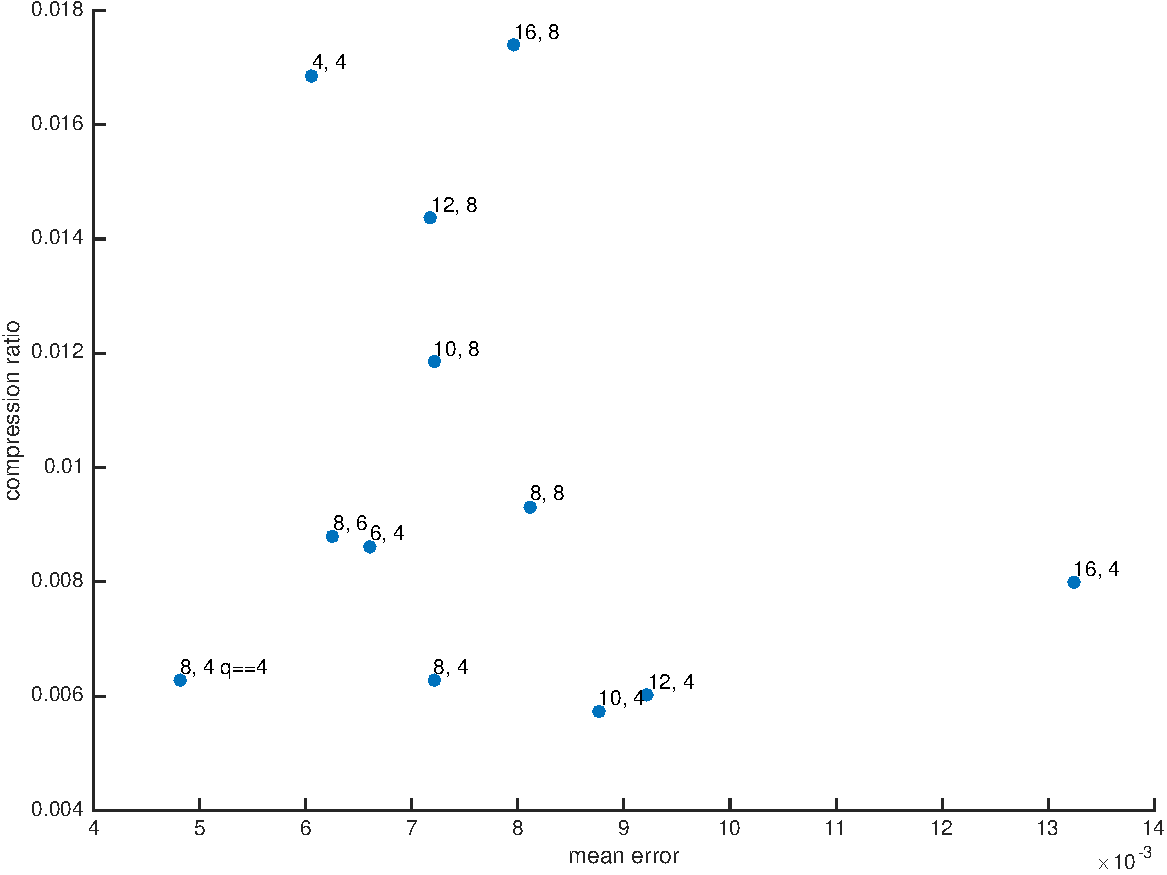
\includegraphics[width=\columnwidth]{images/optParams}
  \caption{Compression ratio and error for different parameters, where the first number of each point is the patch size and the second number is the number of hidden layer nodes in the neural network. For all points but the lower left one the number of quantization bits is 3, and 4 for the lower left point.}
  \label{fig:optParams}
\end{figure}

\newline
To find the optimal parameters the program was executed with different values for the parameters and the results are shown in Figure~\ref{fig:optParams}. There are basically three important parameters: the patch size, the number of hidden layer nodes and the number of quantization bits. The program was executed for patch sizes and number of hidden layer nodes between 4 and 16. The number quantization bits was 3 for the experiments. As the graph shows, the optimal values for patch size and hidden layers were 8 and 4. Setting the number of quantization bits to 4 instead of 3 gave even better results for the mean error.   
% PATCH SIZE 4, HIDDEN LAYERS 4
%Time for everything: 117.5568
%Average quadratic error: 0.0060538
%Average compression rate: 0.016862
%Average inverse for sum compression/error 43.6374

% PATCH SIZE 6, HIDDEN LAYERS 4
%Time for everything: 52.8711
%Average quadratic error: 0.006604
%Average compression rate: 0.0086164
%Average inverse for sum compression/error 65.7015

% PATCH SIZE 8, HIDDEN LAYERS 4
%Time for everything: 30.2464
%Average quadratic error: 0.0072032
%Average compression rate: 0.0062847
%Average inverse for sum compression/error 74.1408

% PATCH SIZE 10, HIDDEN LAYERS 4
%Time for everything: 20.1319
%Average quadratic error: 0.0087594
%Average compression rate: 0.0057288
%Average inverse for sum compression/error 69.0213

% PATCH SIZE 12, HIDDEN LAYERS 4
%Time for everything: 13.5843
%Average quadratic error: 0.0092245
%Average compression rate: 0.0060221
%Average inverse for sum compression/error 65.5884

% PATCH SIZE 16, HIDDEN LAYERS 4
%Time for everything: 7.295
%Average quadratic error: 0.013239
%Average compression rate: 0.0079995
%Average inverse for sum compression/error 47.0841

% PATCH SIZE 8 HIDDEN LAYERS 6
%Time for everything: 42.452
%Average quadratic error: 0.0062569
%Average compression rate: 0.0088015
%Average inverse for sum compression/error 66.4077

% PATCH SIZE 8 HIDDEN LAYERS 8
%Time for everything: 55.9548
%Average quadratic error: 0.008112
%Average compression rate: 0.0093225
%Average inverse for sum compression/error 57.3575

% PATCH SIZE 8 HIDDEN LAYERS 10
%Time for everything: 56.6679
%Average quadratic error: 0.0072036
%Average compression rate: 0.011839
%Average inverse for sum compression/error 52.5127

% PATCH SIZE 8 HIDDEN LAYERS 12
%Time for everything: 70.1564
%Average quadratic error: 0.0071811
%Average compression rate: 0.014356
%Average inverse for sum compression/error 46.4308

% PATCH SIZE 8 HIDDEN LAYERS 16
%Time for everything: 92.5174
%Average quadratic error: 0.0079607
%Average compression rate: 0.017394
%Average inverse for sum compression/error 39.4401

% PATCH SIZE 9 HIDDEN LAYERS 4
%Time for everything: 18.4964
%Average quadratic error: 0.0066528
%Average compression rate: 0.0058509
%Average inverse for sum compression/error 79.9763

% PATCH SIZE 9 HIDDEN LAYERS 5
%Time for everything: 22.764
%Average quadratic error: 0.0072818
%Average compression rate: 0.0061806
%Average inverse for sum compression/error 74.2808

% PATCH SIZE 7 HIDDEN LAYERS 4
%Time for everything: 30.2616
%Average quadratic error: 0.0081324
%Average compression rate: 0.0071031
%Average inverse for sum compression/error 65.6363

% PATCH SIZE 9 HIDDEN LAYERS 4 with QUANTIZATION == 4
%Time for everything: 22.4151
%Average quadratic error: 0.0054932
%Average compression rate: 0.0058509
%Average inverse for sum compression/error 88.1513

% PATCH SIZE 8 HIDDEN LAYERS 4 with QUANTIZATION == 4
%Time for everything: 28.7499
%Average quadratic error: 0.004827
%Average compression rate: 0.0062847
%Average inverse for sum compression/error 89.9952s

% PATCH SIZE 8 HIDDEN LAYERS 4 with QUANTIZATION == 4, Training with 300 samples instead of 100.
%Time for everything: 29.0196
%Average quadratic error: 0.0048096
%Average compression rate: 0.0062847
%Average inverse for sum compression/error 90.1365


\subsection{Comparison to Baselines}


\begin{table}
\centering
    \begin{tabular}{| l | l | l | l |}
    \hline
    Algorithm & Exec. Time & Mean Error & Compr. Ratio \\ \hline
    PCA & 11.56 & 0.000201 & 0.48466\\ \hline
    GMM & 64.93 & 0.011028 & 0.13965 \\ \hline
    NN & 596.42 & 0.008281 & 0.00920 \\
    \hline
    \end{tabular}
    \caption{Numerical comparison of the neural networks algorithm to the baselines. Each algorithm is applied to the same image set with 100 images, which is also the training set for the neural network.}
    \label{tab:compareBaselines}
\end{table}

We compare our solution with two baselines. The first baseline is a compression algorithm based on PCA and the second algorithm is based on Clustering with GMM.  
\newline
In PCA, one projects high dimensional data to low dimensional data. This can be done using the eigenvalue decomposition on the covariance matrix $\Sigma$, which describes the covariance matrix as a product of three matrices U, $\Lambda$ and U$^T$. U contains the eigenvectors of  $\Sigma$ and $\Lambda$ contains the eigenvalues of $\Sigma$. Similar to SVD, one can sort the eigenvalues in decreasing order and then take the k largest of them and the first k columns of U and k columns of U$^T$ to reduce the data which has to be saved. 
\newline

\newline
Clustering is the process of assigning each value x in a data set S to some value x' of a smaller set S'. In image compression one can use this technique to reduce the color space. Each pixel is assigned to one of the RGB values in the smaller color set, i.e. to a cluster. Using mixture models, each pixel can be assigned to more than one cluster with a corresponding probability. In a gaussian mixture model, those values are distributed according to a normal distribution. The second baseline compresses images with this approach. 
\newline
The two baseline algorithms were executed on a the training image set with 100 images from before. For the PCA algorithm, the number of eigenvalues k was chosen to be 100 and the patch size 20, because those values gave the best results in terms of compression ratio and mean error. In GMM, the number of clusters was chosen to be 3 because of the same reason. As Table~\ref{tab:compareBaselines} shows the execution time(Compression and Decompression) of PCA on 100 images was 11.59 seconds and the execution time of GMM was 64.93 seconds. Compared to our neural network algorithm which takes about 600 seconds for 100 images the baselines performed much better in time. But the mean error of our neural network approach is about an order of magnitude better than the mean error of GMM and the compression rate is 2 orders better than both, GMM and PCA.


%PCA 100 images
%Time for everything: 11.5597
%Average quadratic error: 0.00020142
%Average compression rate: 0.48466
%Average inverse for sum compression/error 2.0625

%GMM 100 images
%Time for everything: 64.9339
%Average quadratic error: 0.011028
%Average compression rate: 0.13965
%Average inverse for sum compression/error 6.6365

% Neural net 100 images
%Time for everything: 596.4225
%Average quadratic error: 0.010204
%Average compression rate: 0.0071312
%Average inverse for sum compression/error 57.6857

